% =====================================================================
% 4. Area 2: learning strategies (PRDL, Maria Martinez)
% Shared tasks T13, T14, T24 (OF + MM; DECISIONS D7, D13, D20; block note 08).
% =====================================================================
\section{Area 2: learning strategies}\label{sec:strategies}

The second area asks for a foundational model trained in a self-supervised way, connected to transfer
learning, fine-tuning and zero-shot learning \cite{course_message_2011}. Oriana and I designed and ran
these experiments together (tasks T13, T14 and T24); the generator they reuse is Oriana's
(Section~\ref{sec:generative}). The concepts are summarised in Appendix~\ref{app:strategies}.

\subsection{Self-supervised pre-training and transfer}

\paragraph{Concepts.} Self-supervised learning is ``a feature learning technique for overcoming the
challenges related to the scarcity of `labelled' data'' \cite{soltanieh2022analysis}: the model solves a
pretext task that needs no manual labels and is then reused. The course distinguishes it from transfer
learning by the labels used in pre-training, while noting that both reuse knowledge
\cite{course_summary_0910}. A pre-trained network can be reused in two ways: a linear classifier on its
frozen representation (linear probe), or end-to-end fine-tuning of the whole network
\cite{radford2021learning}. Fine-tuning is usually done with a smaller learning rate ``to prevent
catastrophic forgetting'' \cite{soltanieh2023indistribution}.

\paragraph{Design (decision D20).} Our foundational model is the ECG-GPT of Section~\ref{sec:generative}:
a small causal Transformer trained to predict the next sample of lead II, which is a pretext task without
labels, on the training folds only. Without its next-token head it gives one vector per record. We reused
it on the five superclasses (lead II as input) in three ways: training the same architecture from scratch
(learning rate $10^{-3}$), a linear probe on the frozen network ($10^{-3}$), and fine-tuning with a rate
ten times smaller ($10^{-4}$), as in the class transfer-learning notebook \cite{course_nb_transfer}.
Each was run with 100\,\% and with 10\,\% of the training labels, the 10\,\% subset drawn by patient
(\transferNTrainFinetuneFOneZero{} records). The generator saw the signals of all training records, so
``10\,\%'' means 10\,\% of the labels, not of the data, a semi-supervised setting. Two ablations at the
other learning rate form a $2 \times 2$ of initialisation $\times$ learning rate, to tell whether
fine-tuning wins because of the pre-trained weights or because of the rate.

% Shared float (common/make_floats.py). Table: tables/transfer_main.tex
\begin{table}[htbp]
\centering
\caption[Transfer from the ECG-GPT: main results]{ECG-GPT reused for the five superclasses (lead II): the three strategies with 100\,\% and 10\,\% of the training labels (mean $\pm$ SD over seeds 42--44).}
\label{tab:transfer_main}
\small
\begin{adjustbox}{max width=\textwidth}
% Generated by src/transfer_experiments.py from results/logs/transfer_summary.json.
% Needs report/numbers.tex (alias "transfer") and booktabs.
\begin{tabular}{llrrccc}
\toprule
Labels & Strategy & Train.\ param. & Train records & Val.\ macro AUROC & Test macro AUROC & Test macro F1 \\
\midrule
100\% & From scratch & \transferParamsScratchFOneZeroZero{} & \transferNTrainScratchFOneZeroZero{} & \transferValAurocMeanScratchFOneZeroZero{} $\pm$ \transferValAurocSdScratchFOneZeroZero{} & \transferTestAurocMeanScratchFOneZeroZero{} $\pm$ \transferTestAurocSdScratchFOneZeroZero{} & \transferTestFOneMeanScratchFOneZeroZero{} $\pm$ \transferTestFOneSdScratchFOneZeroZero{} \\
100\% & Linear probe (frozen) & \transferParamsProbeFOneZeroZero{} & \transferNTrainProbeFOneZeroZero{} & \transferValAurocMeanProbeFOneZeroZero{} $\pm$ \transferValAurocSdProbeFOneZeroZero{} & \transferTestAurocMeanProbeFOneZeroZero{} $\pm$ \transferTestAurocSdProbeFOneZeroZero{} & \transferTestFOneMeanProbeFOneZeroZero{} $\pm$ \transferTestFOneSdProbeFOneZeroZero{} \\
100\% & Fine-tuning & \transferParamsFinetuneFOneZeroZero{} & \transferNTrainFinetuneFOneZeroZero{} & \transferValAurocMeanFinetuneFOneZeroZero{} $\pm$ \transferValAurocSdFinetuneFOneZeroZero{} & \transferTestAurocMeanFinetuneFOneZeroZero{} $\pm$ \transferTestAurocSdFinetuneFOneZeroZero{} & \transferTestFOneMeanFinetuneFOneZeroZero{} $\pm$ \transferTestFOneSdFinetuneFOneZeroZero{} \\
\addlinespace
10\% & From scratch & \transferParamsScratchFOneZero{} & \transferNTrainScratchFOneZero{} & \transferValAurocMeanScratchFOneZero{} $\pm$ \transferValAurocSdScratchFOneZero{} & \transferTestAurocMeanScratchFOneZero{} $\pm$ \transferTestAurocSdScratchFOneZero{} & \transferTestFOneMeanScratchFOneZero{} $\pm$ \transferTestFOneSdScratchFOneZero{} \\
10\% & Linear probe (frozen) & \transferParamsProbeFOneZero{} & \transferNTrainProbeFOneZero{} & \transferValAurocMeanProbeFOneZero{} $\pm$ \transferValAurocSdProbeFOneZero{} & \transferTestAurocMeanProbeFOneZero{} $\pm$ \transferTestAurocSdProbeFOneZero{} & \transferTestFOneMeanProbeFOneZero{} $\pm$ \transferTestFOneSdProbeFOneZero{} \\
10\% & Fine-tuning & \transferParamsFinetuneFOneZero{} & \transferNTrainFinetuneFOneZero{} & \transferValAurocMeanFinetuneFOneZero{} $\pm$ \transferValAurocSdFinetuneFOneZero{} & \transferTestAurocMeanFinetuneFOneZero{} $\pm$ \transferTestAurocSdFinetuneFOneZero{} & \transferTestFOneMeanFinetuneFOneZero{} $\pm$ \transferTestFOneSdFinetuneFOneZero{} \\
\bottomrule
\end{tabular}

\end{adjustbox}
\end{table}


\paragraph{Results} (Table~\ref{tab:transfer_main}, Figure~\ref{fig:transfer_strategies}).
\begin{enumerate}[leftmargin=1.4em,itemsep=2pt]
  \item \textbf{Pre-training pays off when the whole network is adapted.} Fine-tuning beats training from
        scratch by \transferTestDiffMeanFinetuneVsScratchFOneZeroZero{} with all the labels and by
        \transferTestDiffMeanFinetuneVsScratchFOneZero{} with 10\,\% of them, in all seeds. The gain
        comes from the pre-trained weights, not from the smaller rate: it remains when scratch is trained
        at the same rate (validation ablation).
  \item \textbf{Label efficiency.} Fine-tuning with 10\,\% of the labels beats training from scratch with
        all of them (\transferTestDiffMeanFinetuneFOneZeroVsScratchFOneZeroZero{}, all seeds). This
        matches the literature on ECG, where the benefit of pre-training ``widens for smaller training
        sets'' \cite{strodthoff2021deep}.
  \item \textbf{The frozen features are weakly diagnostic.} The linear probe is worse than scratch with
        all the labels (\transferTestDiffMeanProbeVsScratchFOneZeroZero{}) and better only with 10\,\%
        (\transferTestDiffMeanProbeVsScratchFOneZero{}). A hypothesis, not tested: predicting the next
        sample rewards local waveform detail more than the global features that separate the classes.
  \item \textbf{A better generator did not give better features.} A linear probe on every other generator
        of the generative block (Figure~\ref{fig:transfer_probe_study}) showed that all of them give better
        frozen features than the one chosen for being the best generator; the rank correlation between
        bits per sample and probe AUROC is positive (\transferProbeSpearmanFOneZeroZero{} with all labels,
        \transferProbeSpearmanFOneZero{} with 10\,\%). The rule that chose the pre-trained model by
        generation quality was fixed in advance and the main experiment keeps it, but in hindsight it was
        not the best rule for transfer. Why fewer bits gave worse features is a hypothesis.
  \item \textbf{Limits.} The ``foundational'' model is very small: it was pre-trained only on the
        training folds of PTB-XL itself. The probe with 10\,\% of the labels reached its best epoch near
        the 50-epoch limit, so it was limited by the epoch budget. Early stopping of the 10\,\% runs used
        the whole validation fold, about as many labelled records as their training subset.
\end{enumerate}

% Shared float (common/make_floats.py). Figure: figures/transfer_strategies.pdf
\begin{figure}[htbp]
\centering
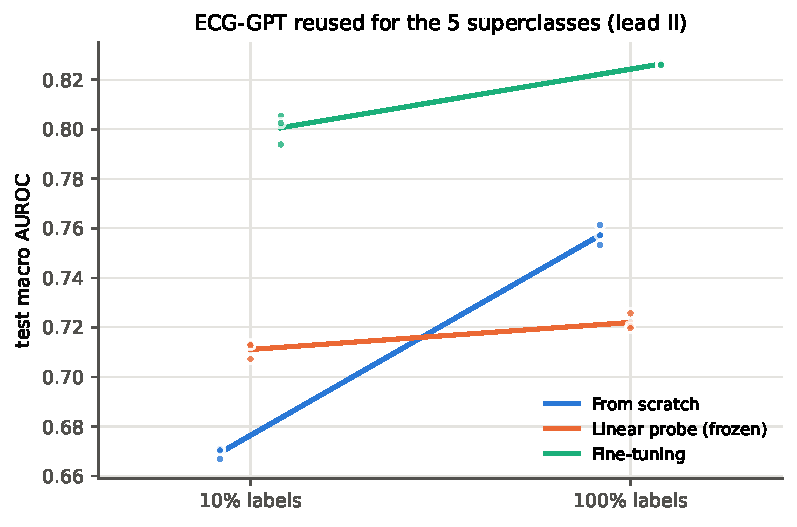
\includegraphics[width=\textwidth,height=0.42\textheight,keepaspectratio]{figures/transfer_strategies.pdf}
\caption[Transfer from the ECG-GPT: strategies and label fractions]{ECG-GPT reused for the five superclasses (lead II): test macro AUROC of training from scratch, linear probe on the frozen network and fine-tuning, with 10\,\% and 100\,\% of the training labels (dots: seeds; line: mean).}
\label{fig:transfer_strategies}
\end{figure}

% Shared float (common/make_floats.py). Figure: figures/transfer_probe_study.pdf
\begin{figure}[htbp]
\centering
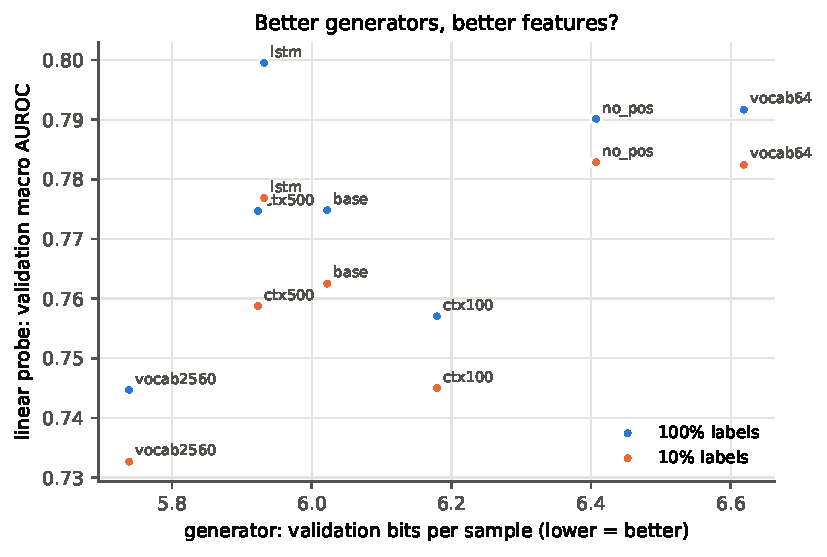
\includegraphics[width=\textwidth,height=0.42\textheight,keepaspectratio]{figures/transfer_probe_study.pdf}
\caption[Probe study: generator quality against feature quality]{Probe study: validation bits per sample of each generator of the generative block against the validation macro AUROC of a linear probe on its frozen features (mean over seeds), with 100\,\% and 10\,\% of the labels.}
\label{fig:transfer_probe_study}
\end{figure}


\paragraph{My reading.} On the same input, the CNN trained from scratch on lead II with all the labels is
still better than the fine-tuned ECG-GPT (\comparisonTestDiffMeanFinetuneFOneZeroZeroVsOneleadCnn{}, all
seeds; Table~\ref{tab:comparison_final}). Pre-training closed most of the gap between the ECG-GPT from
scratch and the CNN, but not all of it. This is the same lesson as in my architecture blocks: on this
dataset size the inductive bias of local filters weighs more than a self-supervised start of a
Transformer.

\subsection{Twelve leads against one lead}

As a cross-cutting ablation, the final model of each family was trained again on lead II only, the input
of the ECG-GPT (Table~\ref{tab:leads}). Every family loses on test, in
all seeds: the dense network \leadsTestDiffMeanDense{}, the CNN \leadsTestDiffMeanCnn{}, the RNN
\leadsTestDiffMeanRnn{}, the RNN + attention \leadsTestDiffMeanRnnattn{} and the Transformer
\leadsTestDiffMeanTransformer{}. The other eleven leads are not redundant with lead II for these
superclasses, and the order of the families barely changes: the CNN stays first and the Transformer last
of the four with shared weights. Part of the explanation is documented: anterior infarction is expressed
``as ST elevation in some or all of leads V1 through V6'' \cite{wagner2009aha}, chest leads that a model
of lead II does not see. That the same holds for hypertrophy is a hypothesis without a source.

% Shared float (common/make_floats.py). Table: tables/leads.tex
\begin{table}[htbp]
\centering
\caption[12 leads against lead II]{12 leads against lead II only, final model of each family (test fold, mean over seeds; $\Delta$ = paired difference, lead II minus 12 leads).}
\label{tab:leads}
\small
\begin{adjustbox}{max width=\textwidth}
% Generated by src/leads_experiments.py from results/logs/leads_summary.json.
% Needs report/numbers.tex (alias "leads") and booktabs.
\begin{tabular}{llrccrc}
\toprule
Family & Final config. & Param.\ (12 / 1) & Test AUROC, 12 leads & Test AUROC, lead II & $\Delta$ & Seeds better / worse \\
\midrule
Dense & \texttt{no\_norm} & \leadsParamsTwelveDense{} / \leadsParamsOneleadDense{} & \leadsTestAurocMeanTwelveDense{} $\pm$ \leadsTestAurocSdTwelveDense{} & \leadsTestAurocMeanOneleadDense{} $\pm$ \leadsTestAurocSdOneleadDense{} & \leadsTestDiffMeanDense{} & \leadsTestNBetterDense{} / \leadsTestNWorseDense{} of \leadsTestNComparedDense{} \\
CNN & \texttt{no\_dropout} & \leadsParamsTwelveCnn{} / \leadsParamsOneleadCnn{} & \leadsTestAurocMeanTwelveCnn{} $\pm$ \leadsTestAurocSdTwelveCnn{} & \leadsTestAurocMeanOneleadCnn{} $\pm$ \leadsTestAurocSdOneleadCnn{} & \leadsTestDiffMeanCnn{} & \leadsTestNBetterCnn{} / \leadsTestNWorseCnn{} of \leadsTestNComparedCnn{} \\
RNN & \texttt{conv} & \leadsParamsTwelveRnn{} / \leadsParamsOneleadRnn{} & \leadsTestAurocMeanTwelveRnn{} $\pm$ \leadsTestAurocSdTwelveRnn{} & \leadsTestAurocMeanOneleadRnn{} $\pm$ \leadsTestAurocSdOneleadRnn{} & \leadsTestDiffMeanRnn{} & \leadsTestNBetterRnn{} / \leadsTestNWorseRnn{} of \leadsTestNComparedRnn{} \\
RNN + attention & \texttt{raw\_attn} & \leadsParamsTwelveRnnattn{} / \leadsParamsOneleadRnnattn{} & \leadsTestAurocMeanTwelveRnnattn{} $\pm$ \leadsTestAurocSdTwelveRnnattn{} & \leadsTestAurocMeanOneleadRnnattn{} $\pm$ \leadsTestAurocSdOneleadRnnattn{} & \leadsTestDiffMeanRnnattn{} & \leadsTestNBetterRnnattn{} / \leadsTestNWorseRnnattn{} of \leadsTestNComparedRnnattn{} \\
Transformer & \texttt{no\_pos} & \leadsParamsTwelveTransformer{} / \leadsParamsOneleadTransformer{} & \leadsTestAurocMeanTwelveTransformer{} $\pm$ \leadsTestAurocSdTwelveTransformer{} & \leadsTestAurocMeanOneleadTransformer{} $\pm$ \leadsTestAurocSdOneleadTransformer{} & \leadsTestDiffMeanTransformer{} & \leadsTestNBetterTransformer{} / \leadsTestNWorseTransformer{} of \leadsTestNComparedTransformer{} \\
\bottomrule
\end{tabular}

\end{adjustbox}
\end{table}


\subsection{Zero-shot learning}

\paragraph{Concept.} In zero-shot classification the model assigns classes it was not trained on with
labels. With other modalities this ``is generally possible thanks to a Multimodal Correspondence'', a
shared embedding space for the inputs and the class descriptions \cite{course_summary_0910}. CLIP builds
one from ``400 million (image, text) pairs'' collected on the Internet \cite{radford2021learning}; it
classifies an image by the cosine similarity between its embedding and the embedding of a sentence for
each class, scaled and passed through a softmax \cite{radford2021learning}. Our ECG-GPT has no text side:
it can be transferred, but not used zero-shot.

\paragraph{Experiment} (decision D20, on the class CLIP notebook \cite{course_nb_clip};
Table~\ref{tab:zeroshot}). On CIFAR-100, where image and text meet in the training data, CLIP picks the
right class among 100 for \zeroshotCifarTopOneNotebook{} of the images (chance \zeroshotCifarChanceTopOne{})
with the notebook's sentence. On lead II of PTB-XL drawn as an image, with one sentence per superclass, all
test images are recognised as ``an electrocardiogram'' among six modality sentences
(\zeroshotFracModalityEcgTestPct{}), but the macro AUROC is only \zeroshotTestMacroAuroc{}
[\zeroshotTestMacroAurocLo{}, \zeroshotTestMacroAurocHi{}], below the trivial model, and the ST-T sentence
wins for \zeroshotFracTopSTTCTestPct{} of the records. CLIP recognises the modality but not the diagnosis.
Why it fails is a hypothesis: the source describes what kind of data CLIP was trained on, not whether ECG
traces with diagnoses are among it.

% Shared float (common/make_floats.py). Table: tables/zeroshot.tex
\begin{table}[htbp]
\centering
\caption[Zero-shot CLIP]{Zero-shot CLIP ViT-B/32: CIFAR-100 (where zero-shot should work) and PTB-XL lead II images (95\,\% bootstrap intervals; patients as the unit on PTB-XL).}
\label{tab:zeroshot}
\small
\begin{adjustbox}{max width=\textwidth}
% Generated by src/zero_shot.py from results/logs/zeroshot.json.
% Needs report/numbers.tex (alias "zeroshot") and booktabs.
\begin{tabular}{llc}
\toprule
Data & Measure & Value [95\% CI] \\
\midrule
CIFAR-100 & top-1 accuracy, ``This is a photo of a \{label\}'' & \zeroshotCifarTopOneNotebook{} [\zeroshotCifarTopOneLoNotebook{}, \zeroshotCifarTopOneHiNotebook{}] \\
CIFAR-100 & top-5 accuracy, ``This is a photo of a \{label\}'' & \zeroshotCifarTopFiveNotebook{} [\zeroshotCifarTopFiveLoNotebook{}, \zeroshotCifarTopFiveHiNotebook{}] \\
CIFAR-100 & top-1 accuracy, bare label & \zeroshotCifarTopOneLabel{} [\zeroshotCifarTopOneLoLabel{}, \zeroshotCifarTopOneHiLabel{}] \\
CIFAR-100 & top-5 accuracy, bare label & \zeroshotCifarTopFiveLabel{} [\zeroshotCifarTopFiveLoLabel{}, \zeroshotCifarTopFiveHiLabel{}] \\
CIFAR-100 & chance (top-1) & \zeroshotCifarChanceTopOne{} \\
\midrule
PTB-XL lead II & images seen as ``an electrocardiogram'' & \zeroshotFracModalityEcgTest{} \\
PTB-XL lead II & macro AUROC, validation & \zeroshotValMacroAuroc{} [\zeroshotValMacroAurocLo{}, \zeroshotValMacroAurocHi{}] \\
PTB-XL lead II & macro AUROC, test & \zeroshotTestMacroAuroc{} [\zeroshotTestMacroAurocLo{}, \zeroshotTestMacroAurocHi{}] \\
PTB-XL lead II & AUROC NORM, test & \zeroshotTestAurocNORM{} [\zeroshotTestAurocNORMLo{}, \zeroshotTestAurocNORMHi{}] \\
PTB-XL lead II & AUROC MI, test & \zeroshotTestAurocMI{} [\zeroshotTestAurocMILo{}, \zeroshotTestAurocMIHi{}] \\
PTB-XL lead II & AUROC STTC, test & \zeroshotTestAurocSTTC{} [\zeroshotTestAurocSTTCLo{}, \zeroshotTestAurocSTTCHi{}] \\
PTB-XL lead II & AUROC CD, test & \zeroshotTestAurocCD{} [\zeroshotTestAurocCDLo{}, \zeroshotTestAurocCDHi{}] \\
PTB-XL lead II & AUROC HYP, test & \zeroshotTestAurocHYP{} [\zeroshotTestAurocHYPLo{}, \zeroshotTestAurocHYPHi{}] \\
\bottomrule
\end{tabular}

\end{adjustbox}
\end{table}

